% Options for packages loaded elsewhere
\PassOptionsToPackage{unicode}{hyperref}
\PassOptionsToPackage{hyphens}{url}
\documentclass[
]{article}
\usepackage{xcolor}
\usepackage{amsmath,amssymb}
\setcounter{secnumdepth}{-\maxdimen} % remove section numbering
\usepackage{iftex}
\ifPDFTeX
  \usepackage[T1]{fontenc}
  \usepackage[utf8]{inputenc}
  \usepackage{textcomp} % provide euro and other symbols
\else % if luatex or xetex
  \usepackage{unicode-math} % this also loads fontspec
  \defaultfontfeatures{Scale=MatchLowercase}
  \defaultfontfeatures[\rmfamily]{Ligatures=TeX,Scale=1}
\fi
\usepackage{lmodern}
\ifPDFTeX\else
  % xetex/luatex font selection
\fi
% Use upquote if available, for straight quotes in verbatim environments
\IfFileExists{upquote.sty}{\usepackage{upquote}}{}
\IfFileExists{microtype.sty}{% use microtype if available
  \usepackage[]{microtype}
  \UseMicrotypeSet[protrusion]{basicmath} % disable protrusion for tt fonts
}{}
\makeatletter
\@ifundefined{KOMAClassName}{% if non-KOMA class
  \IfFileExists{parskip.sty}{%
    \usepackage{parskip}
  }{% else
    \setlength{\parindent}{0pt}
    \setlength{\parskip}{6pt plus 2pt minus 1pt}}
}{% if KOMA class
  \KOMAoptions{parskip=half}}
\makeatother
\usepackage{color}
\usepackage{fancyvrb}
\newcommand{\VerbBar}{|}
\newcommand{\VERB}{\Verb[commandchars=\\\{\}]}
\DefineVerbatimEnvironment{Highlighting}{Verbatim}{commandchars=\\\{\}}
% Add ',fontsize=\small' for more characters per line
\newenvironment{Shaded}{}{}
\newcommand{\AlertTok}[1]{\textcolor[rgb]{1.00,0.00,0.00}{\textbf{#1}}}
\newcommand{\AnnotationTok}[1]{\textcolor[rgb]{0.38,0.63,0.69}{\textbf{\textit{#1}}}}
\newcommand{\AttributeTok}[1]{\textcolor[rgb]{0.49,0.56,0.16}{#1}}
\newcommand{\BaseNTok}[1]{\textcolor[rgb]{0.25,0.63,0.44}{#1}}
\newcommand{\BuiltInTok}[1]{\textcolor[rgb]{0.00,0.50,0.00}{#1}}
\newcommand{\CharTok}[1]{\textcolor[rgb]{0.25,0.44,0.63}{#1}}
\newcommand{\CommentTok}[1]{\textcolor[rgb]{0.38,0.63,0.69}{\textit{#1}}}
\newcommand{\CommentVarTok}[1]{\textcolor[rgb]{0.38,0.63,0.69}{\textbf{\textit{#1}}}}
\newcommand{\ConstantTok}[1]{\textcolor[rgb]{0.53,0.00,0.00}{#1}}
\newcommand{\ControlFlowTok}[1]{\textcolor[rgb]{0.00,0.44,0.13}{\textbf{#1}}}
\newcommand{\DataTypeTok}[1]{\textcolor[rgb]{0.56,0.13,0.00}{#1}}
\newcommand{\DecValTok}[1]{\textcolor[rgb]{0.25,0.63,0.44}{#1}}
\newcommand{\DocumentationTok}[1]{\textcolor[rgb]{0.73,0.13,0.13}{\textit{#1}}}
\newcommand{\ErrorTok}[1]{\textcolor[rgb]{1.00,0.00,0.00}{\textbf{#1}}}
\newcommand{\ExtensionTok}[1]{#1}
\newcommand{\FloatTok}[1]{\textcolor[rgb]{0.25,0.63,0.44}{#1}}
\newcommand{\FunctionTok}[1]{\textcolor[rgb]{0.02,0.16,0.49}{#1}}
\newcommand{\ImportTok}[1]{\textcolor[rgb]{0.00,0.50,0.00}{\textbf{#1}}}
\newcommand{\InformationTok}[1]{\textcolor[rgb]{0.38,0.63,0.69}{\textbf{\textit{#1}}}}
\newcommand{\KeywordTok}[1]{\textcolor[rgb]{0.00,0.44,0.13}{\textbf{#1}}}
\newcommand{\NormalTok}[1]{#1}
\newcommand{\OperatorTok}[1]{\textcolor[rgb]{0.40,0.40,0.40}{#1}}
\newcommand{\OtherTok}[1]{\textcolor[rgb]{0.00,0.44,0.13}{#1}}
\newcommand{\PreprocessorTok}[1]{\textcolor[rgb]{0.74,0.48,0.00}{#1}}
\newcommand{\RegionMarkerTok}[1]{#1}
\newcommand{\SpecialCharTok}[1]{\textcolor[rgb]{0.25,0.44,0.63}{#1}}
\newcommand{\SpecialStringTok}[1]{\textcolor[rgb]{0.73,0.40,0.53}{#1}}
\newcommand{\StringTok}[1]{\textcolor[rgb]{0.25,0.44,0.63}{#1}}
\newcommand{\VariableTok}[1]{\textcolor[rgb]{0.10,0.09,0.49}{#1}}
\newcommand{\VerbatimStringTok}[1]{\textcolor[rgb]{0.25,0.44,0.63}{#1}}
\newcommand{\WarningTok}[1]{\textcolor[rgb]{0.38,0.63,0.69}{\textbf{\textit{#1}}}}
\usepackage{longtable,booktabs,array}
\newcounter{none} % for unnumbered tables
\usepackage{calc} % for calculating minipage widths
% Correct order of tables after \paragraph or \subparagraph
\usepackage{etoolbox}
\makeatletter
\patchcmd\longtable{\par}{\if@noskipsec\mbox{}\fi\par}{}{}
\makeatother
% Allow footnotes in longtable head/foot
\IfFileExists{footnotehyper.sty}{\usepackage{footnotehyper}}{\usepackage{footnote}}
\makesavenoteenv{longtable}
\usepackage{graphicx}
\makeatletter
\newsavebox\pandoc@box
\newcommand*\pandocbounded[1]{% scales image to fit in text height/width
  \sbox\pandoc@box{#1}%
  \Gscale@div\@tempa{\textheight}{\dimexpr\ht\pandoc@box+\dp\pandoc@box\relax}%
  \Gscale@div\@tempb{\linewidth}{\wd\pandoc@box}%
  \ifdim\@tempb\p@<\@tempa\p@\let\@tempa\@tempb\fi% select the smaller of both
  \ifdim\@tempa\p@<\p@\scalebox{\@tempa}{\usebox\pandoc@box}%
  \else\usebox{\pandoc@box}%
  \fi%
}
% Set default figure placement to htbp
\def\fps@figure{htbp}
\makeatother
\usepackage{svg}
\setlength{\emergencystretch}{3em} % prevent overfull lines
\providecommand{\tightlist}{%
  \setlength{\itemsep}{0pt}\setlength{\parskip}{0pt}}
\usepackage{bookmark}
\IfFileExists{xurl.sty}{\usepackage{xurl}}{} % add URL line breaks if available
\urlstyle{same}
\hypersetup{
  hidelinks,
  pdfcreator={LaTeX via pandoc}}

\author{}
\date{}

\begin{document}

\section{Paper 4: Splitting of Reciprocal Dual Cells and Hierarchical
State
Structure}\label{paper-4-splitting-of-reciprocal-dual-cells-and-hierarchical-state-structure}

\subsection{\texorpdfstring{A Minimal Observational Model of Internal
State Capacity, Volume Gap, and Duality Breaking from
\(\nu\lambda=1\)}{A Minimal Observational Model of Internal State Capacity, Volume Gap, and Duality Breaking from \textbackslash nu\textbackslash lambda=1}}\label{a-minimal-observational-model-of-internal-state-capacity-volume-gap-and-duality-breaking-from-nulambda1}

Author: Noriaki Kihara\\
Affiliation: WF System Co., Ltd.\\
ORCID: 0009-0004-6753-4020\\
Version: v1.0\\
Date: June 2026\\
DOI (this version): 10.5281/zenodo.20638963\\
Concept DOI: 10.5281/zenodo.20638962\\
License: CC BY 4.0

\begin{center}\rule{0.5\linewidth}{0.5pt}\end{center}

\subsection{Abstract}\label{abstract}

In this paper, starting from the minimal reciprocal dual condition
placed between wavelength components \(\lambda_n\) and frequency
components \(\nu_n\),

\[
\lambda_n\nu_n=1,
\]

we reconstruct, as a single minimal observational model, the wavelength
space, the frequency space, the 4-dimensional lattice cell counting, and
the closed 4-dimensional structure treated in the three preceding
observational papers.

The purpose of this paper is not to replace standard physical theory,
general relativity, quantum theory, particle physics, or cosmology. Nor
does this paper claim to have derived spacetime, mass, energy,
interactions, the Standard Model, quantum gravity, or a grand unified
theory. The \(\lambda_n\) and \(\nu_n\) treated in this paper are model
variables for observing the dual geometric structure of wavelength space
and frequency space.

In this paper we show that, when the possible existence of a minimal
conjugate width \(\delta_{\min}\) is added to the reciprocal dual
condition, a state is treated not as a mathematical point but as a
conjugate cell with a minimal width. In this case, the composite
frequency radius

\[
R^2=\sum_n \nu_n^2
\]

can be read not as a substantive radius given from outside, but as an
energy-like scale determined from the internal frequency components.
\(R=1\) is observed as the minimal conjugate cell, \(R=2\) as eight
first-neighbor quasi-ground states, and \(R=3\) as a large internal
state shell containing 128 additional states.

Furthermore, by comparing the 4-dimensional hyperball volume

\[
V_4(R)=\frac{\pi^2}{2}R^4
\]

with the fully-inscribed cell volume \(N_0(R)\), we confirm that the
filling fraction shows an asymptotically increasing tendency accompanied
by local fluctuations, while the volume gap as an absolute quantity,

\[
\Delta V(R)=V_4(R)-N_0(R),
\]

grows. From this observation, we introduce a toy model that reads a
single state with high \(R\) as a decomposition into many finite-\(R'\)
states.

Finally, we describe an observation of duality breaking: in the initial
state the roles of \(\nu\) and \(\lambda\) are undifferentiated, and
through the splitting into finite-\(R'\) cells and the minimal conjugate
width, the frequency side differentiates into dense internal states
while the wavelength side differentiates into a sparse extension. This
observation does not derive the differentiation of time and space.
However, it does serve as a toy model in which the \(\nu\) side is read
as internal updating and state density, and the \(\lambda\) side as
extension and spread.

The conclusion of this paper is that, from the minimal reciprocal dual
assumption \(\nu\lambda=1\), the minimal conjugate cell, internal state
capacity, volume gap, finite-\(R'\) decomposition, duality breaking, and
curved hierarchical structure can be read in a chained manner within the
same observational model.

\begin{center}\rule{0.5\linewidth}{0.5pt}\end{center}

\subsection{Keywords}\label{keywords}

wavelength space, frequency space, reciprocal duality, \(\nu\lambda=1\),
conjugate cell, minimal fluctuation width, 4-dimensional lattice,
4-dimensional hyperball, internal state capacity, volume gap, splitting
representation, duality breaking, central projection, curved state
space, self-similar hierarchy, toy model

\begin{center}\rule{0.5\linewidth}{0.5pt}\end{center}

\subsection{1. Introduction}\label{introduction}

In the preceding Paper 1, we placed between wavelength space and
frequency space the reciprocal dual condition

\[
\lambda_n=\frac{1}{\nu_n},
\]

and observed that, when a constant sum-of-squares condition is further
imposed on the wavelength space and the frequency space, a system of 5
components with 1 constraint retains 4 degrees of freedom. We also
confirmed that, in the logarithmic variables

\[
q_n=\log\lambda_n,\qquad p_n=\log\nu_n,
\]

the reciprocal dual condition is expressed as the sign-reversal symmetry

\[
p_n=-q_n.
\]

In the preceding Paper 2, we formulated the unit-cell counting on the
4-dimensional integer lattice and computed the number \(N_0(R)\) of unit
cells fully inscribed in a 4-dimensional hyperball of radius \(R\). In
particular, we confirmed that the values

\[
N_0(1)=1,\qquad N_0(2)=9,\qquad N_0(3)=137
\]

are obtained.

In the preceding Paper 3, we provided a supplement connecting this
4-dimensional lattice counting with the closed 4-dimensional structure
and with central-projection-like observation.

In this paper, we reconstruct these three observations from smaller
assumptions. The central assumption is the componentwise reciprocal
duality

\[
\lambda_n\nu_n=1.
\]

In this paper we read this condition not as a mere algebraic relation,
but as the minimal dual structure placed between wavelength space and
frequency space.

The question of this paper can be stated as follows.

\begin{quote}
When a minimal conjugate width, 4-dimensional cell counting, and the
composite radius \(R^2=\sum_n\nu_n^2\) are added to the minimal dual
condition \(\nu\lambda=1\), what internal state structure, volume gap,
splitting representation, and duality breaking are observed?
\end{quote}

In this paper, we treat these not as a physical theory but as an
observational model. Therefore, terms in this paper such as
``energy-like,'' ``ground,'' ``quasi-ground,'' ``splitting,''
``vacuum,'' and ``symmetry breaking'' are not identified with the
concepts of the same names in standard physics. They are restricted
terms for describing the geometric behavior of wavelength-frequency dual
cells.

\begin{center}\rule{0.5\linewidth}{0.5pt}\end{center}

\subsection{2. Related Work and Positioning of This
Paper}\label{related-work-and-positioning-of-this-paper}

The problem awareness of this paper has, in part of its problem setting,
associative points of contact with the body of research that does not
regard spacetime as a background given from the start, but considers the
possibility that spacetime and geometry emerge from more fundamental
discrete structures, relational structures, quantum states, or
pregeometric structures.

In causal set theory, instead of a spacetime continuum, a locally finite
partially ordered set is taken as the foundation, with the order
relation treated as primitive causality and local finiteness as
discreteness {[}Surya 2019{]}. In Quantum Graphity, the possibility is
examined that in the high-energy phase a highly connected graph state
with permutation symmetry exists, while in the low-energy phase the
symmetry is broken and low-dimensional, local structure appears
{[}Konopka and Markopoulou 2006; Konopka, Markopoulou and Severini
2008{]}. In Group Field Theory condensate cosmology, the possibility is
discussed that continuous cosmological dynamics emerges from condensate
states of non-spatiotemporal quantum building blocks {[}Oriti 2021;
Pithis and Sakellariadou 2019{]}. In the context of pregeometry, the
possibility is also discussed that the difference between time and space
is not built in from the start but appears as a result of spontaneous
symmetry breaking {[}Wetterich 2021{]}. The standpoint that reads the
quantum vacuum as a condensed-matter-like medium is also instructive for
thinking of the vacuum not as a structureless void but as a state with
internal degrees of freedom {[}Volovik 2003{]}.

However, this paper does not extend, modify, or unify these existing
theories. The structure of this paper is more restricted. Namely,
starting from the reciprocal dual condition

\[
\lambda_n\nu_n=1,
\]

we investigate what observational structures appear when a minimal
conjugate width, 4-dimensional lattice cell counting, the volume gap,
and the possibility of decomposition into finite-radius cells are added
to it.

Therefore, the positioning of this paper is not that of a candidate for
existing quantum gravity theories or unified theories, but a
\textbf{minimal toy observation model based on wavelength-frequency
duality}.

\begin{center}\rule{0.5\linewidth}{0.5pt}\end{center}

\subsection{3. Basic Assumptions}\label{basic-assumptions}

\subsubsection{3.1 Reciprocal dual
condition}\label{reciprocal-dual-condition}

In this paper, for each component we impose

\[
\lambda_n\nu_n=1,
\]

where \(\lambda_n\) is a component on the wavelength-space side and
\(\nu_n\) is a component on the frequency-space side.

In this paper, we do not identify \(\lambda_n\) and \(\nu_n\) with
spatial coordinates, temporal frequencies, energy, momentum, or other
quantities in standard physics. They are two dual variables in mutual
reciprocal relation.

\subsubsection{3.2 Composite frequency
radius}\label{composite-frequency-radius}

On the frequency-space side, we define the composite radius

\[
R^2=\sum_{n=1}^{d}\nu_n^2,
\]

where \(d\) is the number of frequency components; in this paper we
treat \(d=4\), corresponding to the 4 degrees of freedom left by the
5-component, 1-constraint system of the preceding Paper 1 (§4.1).

In this paper, we treat \(R\) not as a substantive radius given from
outside, but as a composite quantity determined from the sum of squares
of the internal frequency components. In this sense, \(R\) can be read
as an energy-like scale, or as a model label expressing the size of the
internal frequency state.

However, in this paper we do not identify \(R\) with physical energy,
mass, curvature radius, cosmic radius, or the like.

\subsubsection{3.3 Minimal conjugate
width}\label{minimal-conjugate-width}

Ideally,

\[
\lambda_n\nu_n=1,
\]

but if an observed state is treated as a perfect mathematical point,
there is no room left to treat 4-dimensional lattice cell counting or
splitting representations. Therefore, in this paper we assume the
possible existence of a minimal conjugate width:

\[
\delta^2\ge \delta_{\min}^2,
\]

where \(\delta\) is a model quantity expressing the observational or
constitutive width possessed by a wavelength-frequency dual cell. In
this paper we do not derive the value of \(\delta_{\min}\). Where
needed, we use \(\delta_{\min}^2=1/2\) as an illustrative value, but
this is not a physical constant; it is a placeholder to indicate the
scale of the discussion.

\subsubsection{3.4 States are conjugate cells, not
points}\label{states-are-conjugate-cells-not-points}

From the above, in this paper a state is treated not as a point

\[
(\lambda,\nu)
\]

but as a conjugate cell centered on the reciprocal dual condition and
possessing the minimal width \(\delta_{\min}\).

Therefore, the \(R=1\) state is also not a single point

\[
\nu=1,\qquad \lambda=1,
\]

but the minimal conjugate cell centered at \(\nu=1,\lambda=1\).

\begin{center}\rule{0.5\linewidth}{0.5pt}\end{center}

\subsection{\texorpdfstring{4. State Capacity at
\(R=1,2,3\)}{4. State Capacity at R=1,2,3}}\label{state-capacity-at-r123}

\subsubsection{4.1 Fully-inscribed cell count in 4
dimensions}\label{fully-inscribed-cell-count-in-4-dimensions}

In the preceding Papers 1 and 3, we confirmed that the 5-component,
1-constraint system can be read as a closed structure with 4 degrees of
freedom. In this section, as the counting region corresponding to those
4 degrees of freedom, we consider the same 4-dimensional integer lattice
as in the preceding Paper 2:

\[
k=(k_1,k_2,k_3,k_4)\in\mathbb{Z}^4.
\]

A 4-dimensional unit cell of side 1 is associated with each lattice
point \(k\). The half-width of this unit cell along each axis is
\(1/2\); this does not derive the value of \(\delta_{\min}\) of the
previous section, but means that we use the unit-cell normalization of
Paper 2. The condition for this unit cell to be fully inscribed in a
4-dimensional hyperball of radius \(R\) is

\[
\sum_{i=1}^{4}\left(|k_i|+\frac12\right)^2\le R^2.
\]

Therefore, we define the fully-inscribed cell count as

\[
N_0(R)=\#\left\{k\in\mathbb{Z}^4\mid
\sum_{i=1}^{4}\left(|k_i|+\frac12\right)^2\le R^2
\right\}.
\]

Here \(N_0(R)\) is not a particle number. Nor is it the number of
material cells filling real space. \(N_0(R)\) is the geometric capacity
for placing unit cells without overlap inside the model state space of
radius \(R\).

\subsubsection{4.2 State capacity at small
radii}\label{state-capacity-at-small-radii}

Based on the counting of the preceding Paper 2, at integer radii
\(R=1,2,3\) we obtain

\[
N_0(1)=1,
\]

\[
N_0(2)=9,
\]

\[
N_0(3)=137.
\]

Therefore the shell differences are

\[
\Delta N_0(2)=N_0(2)-N_0(1)=8,
\]

\[
\Delta N_0(3)=N_0(3)-N_0(2)=128.
\]

In the toy model of this paper, this sequence can be read as follows.

\begin{itemize}
\tightlist
\item
  \(R=1\) is a ground-like state corresponding to one minimal conjugate
  cell.
\item
  \(R=2\) is a state in which, in addition to the central cell,
  first-neighbor cells appear in the 8 positive and negative directions
  of the 4-dimensional lattice.
\item
  \(R=3\) is a state in which 128 further cells are added, and a large
  internal state shell appears that goes beyond the simple
  first-neighbor shell.
\end{itemize}

\begin{figure}
\centering
\pandocbounded{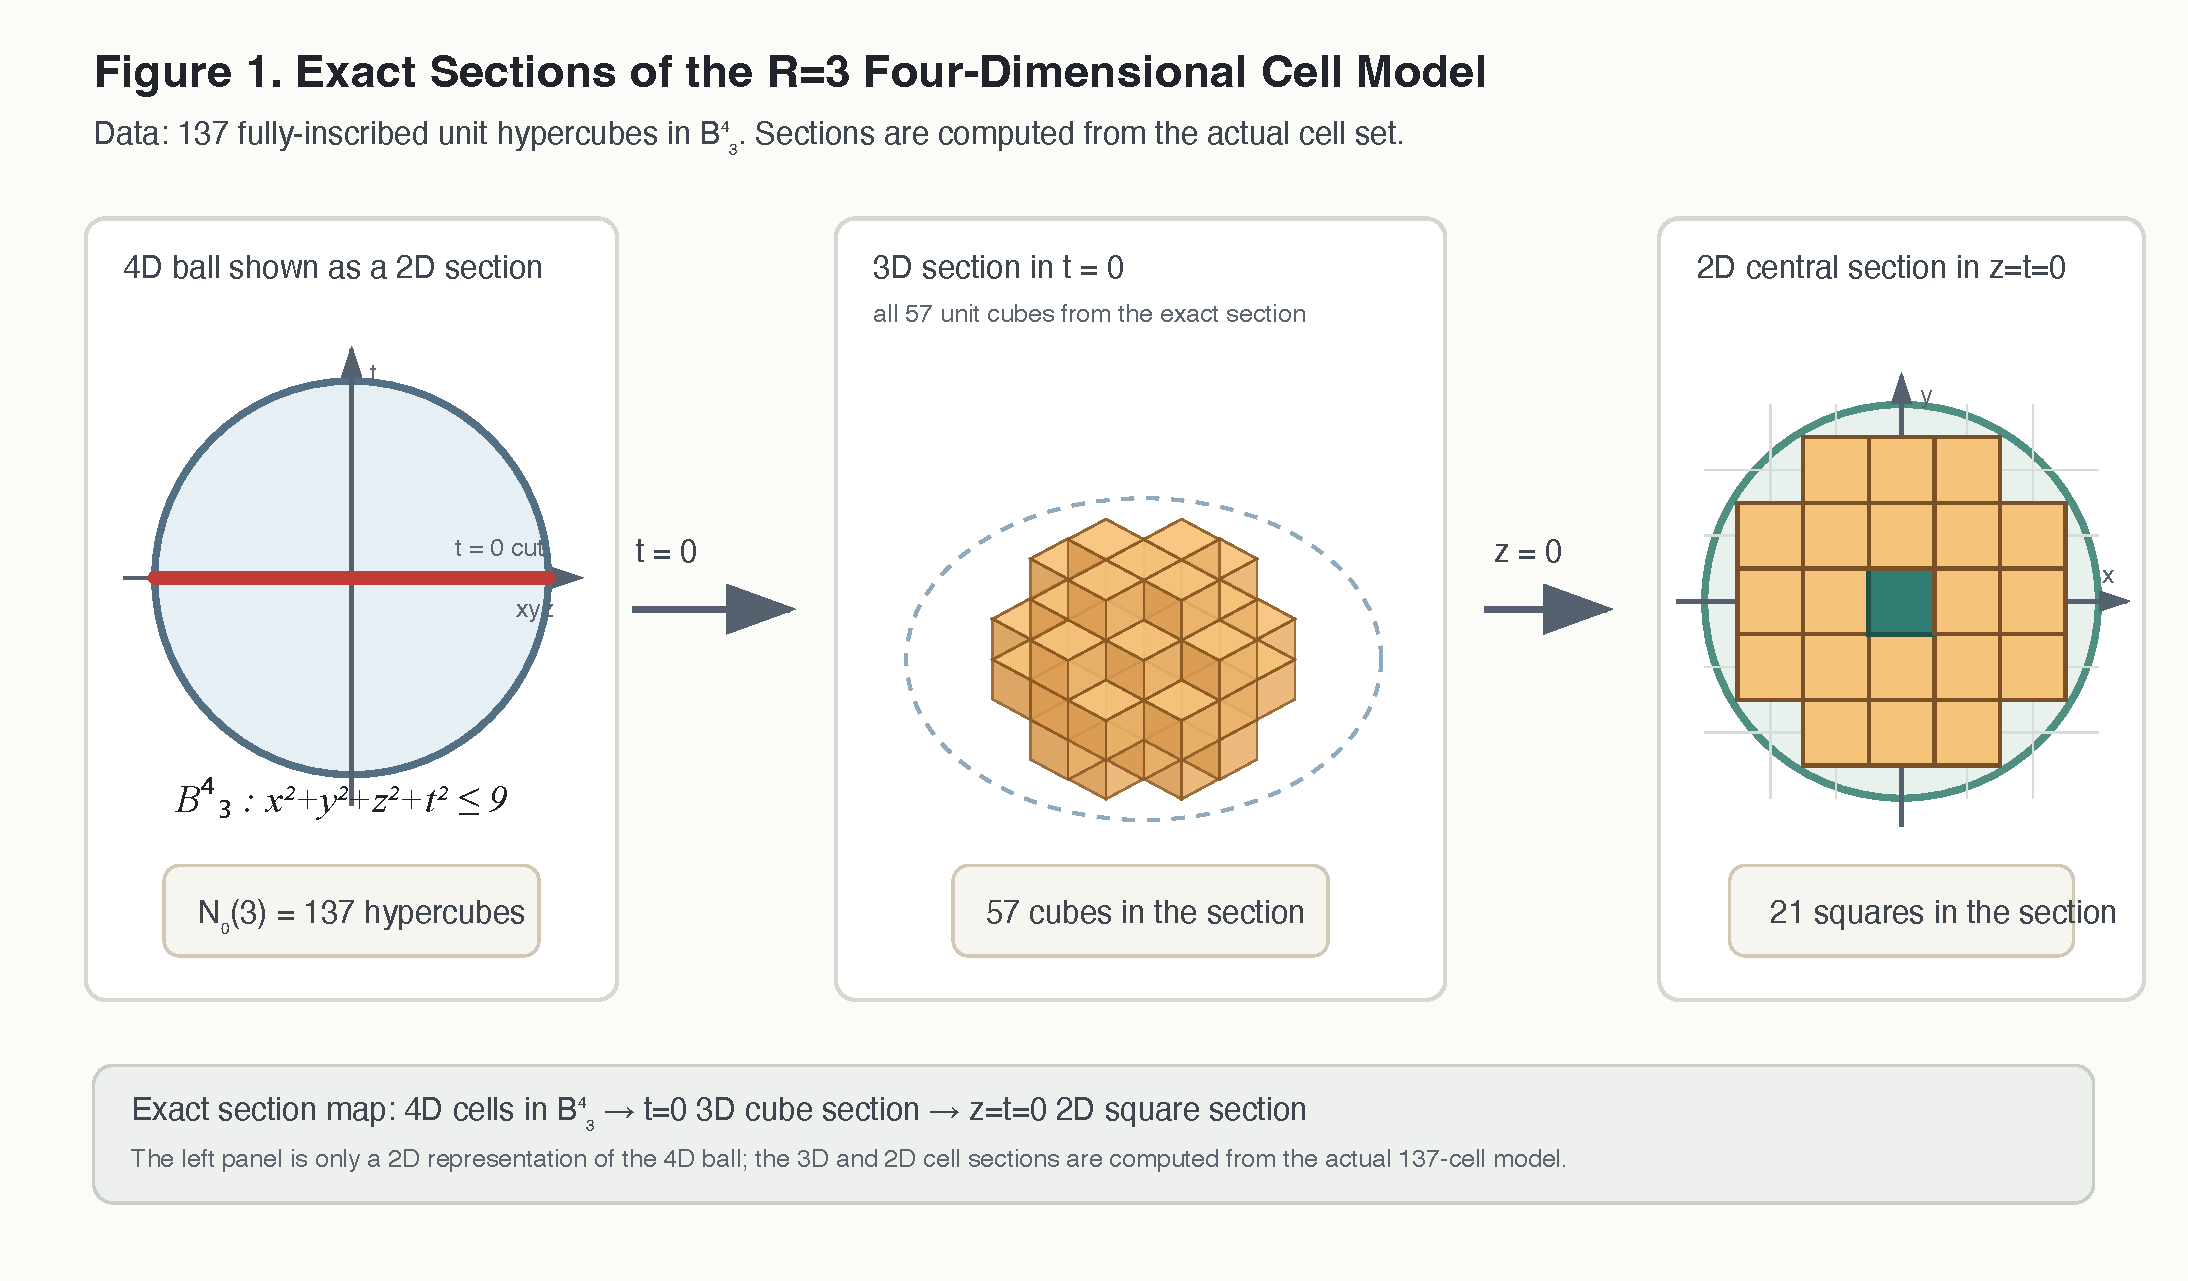
\includegraphics[keepaspectratio]{figure_paper4_1_reciprocal_dual_shell_growth.pdf}}
\caption{Figure 1. Exact Sections of the R=3 Four-Dimensional Cell
Model}
\end{figure}

\textbf{Figure 1. Exact sections of the \(R=3\) four-dimensional cell
model.} We first enumerate the 137 four-dimensional hypercubes of side 1
fully inscribed in the 4-dimensional hyperball \(B^4_3\) of radius
\(R=3\); cutting this cell set at \(t=0\) yields 57 three-dimensional
cubic sections. Cutting further at \(z=0\) yields 21 unit-square
sections on the central two-dimensional plane. The two-dimensional
diagram at the right end is not a schematic shell diagram but the
central section actually obtained from the set of 137 four-dimensional
cells.

\subsubsection{4.3 State capacity table}\label{state-capacity-table}

{\def\LTcaptype{none} % do not increment counter
\begin{longtable}[]{@{}
  >{\raggedleft\arraybackslash}p{(\linewidth - 6\tabcolsep) * \real{0.2667}}
  >{\raggedleft\arraybackslash}p{(\linewidth - 6\tabcolsep) * \real{0.2667}}
  >{\raggedleft\arraybackslash}p{(\linewidth - 6\tabcolsep) * \real{0.2667}}
  >{\raggedright\arraybackslash}p{(\linewidth - 6\tabcolsep) * \real{0.2000}}@{}}
\toprule\noalign{}
\begin{minipage}[b]{\linewidth}\raggedleft
\(R\)
\end{minipage} & \begin{minipage}[b]{\linewidth}\raggedleft
\(N_0(R)\)
\end{minipage} & \begin{minipage}[b]{\linewidth}\raggedleft
Shell difference \(\Delta N_0(R)=N_0(R)-N_0(R-1)\)
\end{minipage} & \begin{minipage}[b]{\linewidth}\raggedright
Reading
\end{minipage} \\
\midrule\noalign{}
\endhead
\bottomrule\noalign{}
\endlastfoot
1 & 1 & 1 & Minimal conjugate cell, ground-like state \\
2 & 9 & 8 & First-neighbor shell, 8 quasi-ground directional states \\
3 & 137 & 128 & Large internal state shell, 128 additional states \\
4 & 473 & 336 & Higher shell including composite directions \\
5 & 1,545 & 1,072 & Growth of internal state capacity \\
6 & 3,457 & 1,912 & Higher internal state capacity \\
7 & 7,281 & 3,824 & Higher internal state capacity \\
8 & 12,833 & 5,552 & Higher internal state capacity \\
9 & 22,409 & 9,576 & Higher internal state capacity \\
10 & 34,569 & 12,160 & Higher internal state capacity \\
\end{longtable}
}

What this table shows is that the internal state capacity grows rapidly
as \(R\) increases. However, rather than interpreting each state as
superposed on the same physical point, we read them as unit cells with
distinct position labels or phase labels in the model state space.

\subsubsection{4.4 Classical reading and state-theoretic
reading}\label{classical-reading-and-state-theoretic-reading}

Classically, the 8 states added at \(R=2\) can be read as minimal orbit
candidates appearing around the central state. On the 4-dimensional
lattice, these correspond to the positive and negative directions of
each of the 4 axes.

State-theoretically, the same 8 can be read as quasi-ground states of
the first shell adjacent to the ground cell.

The 128 states added at \(R=3\) can be read as a large internal state
shell that includes not only single-axis directions but also
combinatorial states spanning multiple axes. However, in this paper we
do not identify them with multiplets of physical particles, spin, gauge
degrees of freedom, particle species of the Standard Model, or the like.

\begin{center}\rule{0.5\linewidth}{0.5pt}\end{center}

\subsection{5. Volume Gap and
Consistency}\label{volume-gap-and-consistency}

\subsubsection{5.1 4-dimensional hyperball
volume}\label{dimensional-hyperball-volume}

The volume of the 4-dimensional hyperball is

\[
V_4(R)=\frac{\pi^2}{2}R^4.
\]

On the other hand, since the fully-inscribed cells are 4-dimensional
unit cells of side 1, the stacked cell volume is

\[
V_{\mathrm{cell}}(R)=N_0(R).
\]

Therefore, we define the difference between the continuous 4-dimensional
hyperball volume and the discrete cell volume as

\[
\Delta V(R)=V_4(R)-N_0(R),
\]

and define the filling fraction as

\[
\eta(R)=\frac{N_0(R)}{V_4(R)}.
\]

\subsubsection{5.2 Volume comparison
table}\label{volume-comparison-table}

{\def\LTcaptype{none} % do not increment counter
\begin{longtable}[]{@{}
  >{\raggedleft\arraybackslash}p{(\linewidth - 8\tabcolsep) * \real{0.2000}}
  >{\raggedleft\arraybackslash}p{(\linewidth - 8\tabcolsep) * \real{0.2000}}
  >{\raggedleft\arraybackslash}p{(\linewidth - 8\tabcolsep) * \real{0.2000}}
  >{\raggedleft\arraybackslash}p{(\linewidth - 8\tabcolsep) * \real{0.2000}}
  >{\raggedleft\arraybackslash}p{(\linewidth - 8\tabcolsep) * \real{0.2000}}@{}}
\toprule\noalign{}
\begin{minipage}[b]{\linewidth}\raggedleft
\(R\)
\end{minipage} & \begin{minipage}[b]{\linewidth}\raggedleft
\(N_0(R)\)
\end{minipage} & \begin{minipage}[b]{\linewidth}\raggedleft
\(V_4(R)=\frac{\pi^2}{2}R^4\)
\end{minipage} & \begin{minipage}[b]{\linewidth}\raggedleft
\(\Delta V(R)=V_4(R)-N_0(R)\)
\end{minipage} & \begin{minipage}[b]{\linewidth}\raggedleft
\(\eta(R)=N_0(R)/V_4(R)\)
\end{minipage} \\
\midrule\noalign{}
\endhead
\bottomrule\noalign{}
\endlastfoot
1 & 1 & 4.9348 & 3.9348 & 0.2026 \\
2 & 9 & 78.9568 & 69.9568 & 0.1140 \\
3 & 137 & 399.7190 & 262.7190 & 0.3427 \\
4 & 473 & 1263.3094 & 790.3094 & 0.3744 \\
5 & 1,545 & 3084.2514 & 1539.2514 & 0.5009 \\
6 & 3,457 & 6395.5037 & 2938.5037 & 0.5405 \\
7 & 7,281 & 11848.4601 & 4567.4601 & 0.6145 \\
8 & 12,833 & 20212.9498 & 7379.9498 & 0.6349 \\
9 & 22,409 & 32377.2372 & 9968.2372 & 0.6921 \\
10 & 34,569 & 49348.0220 & 14779.0220 & 0.7005 \\
\end{longtable}
}

From this table, two observations are obtained.

First, the filling fraction \(\eta(R)\) shows local increases and
decreases, but in the radius sweep of the preceding Paper 2 it shows a
tendency to approach the continuous 4-dimensional hyperball volume at
sufficiently large \(R\).

Second, the volume gap \(\Delta V(R)\) as an absolute quantity grows.
This is because the unfilled region remaining in the fully-inscribed
cell counting corresponds to the boundary layer of the 4-dimensional
hyperball, and its dominant scale is given by the surface area of the
4-dimensional ball, that is, the \(R^3\) order. Therefore, while the
system appears to approach the continuum in relative terms, the absolute
amount of mismatch remains as a boundary-layer scale.

This observation is important. For if one reads a state as a single
state with high \(R\), the internal state capacity becomes large, but at
the same time the difference between the continuous hyperball volume and
the discrete cell volume also becomes large.

\subsubsection{5.3 On the boundary layer and asymptotic
order}\label{on-the-boundary-layer-and-asymptotic-order}

The \(\Delta V(R)\) defined in this paper is the direct difference
between the volume of the 4-dimensional hyperball of the same radius
\(R\) and the fully-inscribed cell volume. This direct difference
includes the unfilled layer near the boundary. The boundary-layer volume
of a 4-dimensional ball of radius \(R\), if the thickness is fixed at
about the unit-cell width, is proportional to the surface-area scale of
the 4-dimensional ball. The surface area of the 4-dimensional ball is

\[
\frac{d}{dR}V_4(R)=\frac{d}{dR}\left(\frac{\pi^2}{2}R^4\right)=2\pi^2R^3,
\]

so the dominant scale of the volume gap is of order \(R^3\).

In this paper, we do not treat the asymptotic constant of
\(\Delta V(R)\) or a detailed evaluation of lattice fluctuations. The
observation needed here is that, even as the filling fraction increases,
the volume gap as an absolute quantity remains as a
boundary-layer-derived quantity of order \(R^3\).

\subsubsection{5.4 Reading the volume gap as a mismatch
indicator}\label{reading-the-volume-gap-as-a-mismatch-indicator}

In this paper, we tentatively read \(\Delta V(R)\) as a mismatch
quantity, or as an indicator for measuring geometric consistency.

In this reading, as \(R\) becomes larger the state capacity increases,
but at the same time the mismatch quantity viewed as a single high-\(R\)
state also increases. Therefore, as far as this indicator alone is
concerned, there are cases where a representation decomposed into many
low-\(R'\) states has a smaller mismatch quantity than a single state
with high \(R\).

However, this consistency is not identified with thermodynamic
stability, quantum mechanical stability, or vacuum stability in field
theory. It is strictly a geometric comparison indicator within this
model.

\begin{center}\rule{0.5\linewidth}{0.5pt}\end{center}

\subsection{\texorpdfstring{6. Splitting into Finite-\(R'\)
States}{6. Splitting into Finite-R\textquotesingle{} States}}\label{splitting-into-finite-r-states}

\subsubsection{\texorpdfstring{6.1 \(R^2\) as the conserved
quantity}{6.1 R\^{}2 as the conserved quantity}}\label{r2-as-the-conserved-quantity}

In this paper, as the quantity conserved before and after splitting, we
consider not \(R\) but \(R^2\). That is, when a single state \(R\) is
decomposed into multiple finite states \(R'_a\), we assume

\[
R^2=\sum_a {R'_a}^2.
\]

This is because \(R^2\) is defined as

\[
R^2=\sum_n\nu_n^2.
\]

That is, \(R^2\) is the sum of squares of frequency components, and it
is natural to read it as a distributable energy-like quantity.

\subsubsection{6.2 Condition favoring
splitting}\label{condition-favoring-splitting}

Let the mismatch quantity of the single state be \(\Delta V(R)\), and
let the mismatch quantity after splitting be

\[
\sum_a \Delta V(R'_a).
\]

Then, if

\[
\Delta V(R)>\sum_a\Delta V(R'_a),
\]

the mismatch quantity after splitting is smaller from the viewpoint of
the volume gap.

For example, considering the single state \(R=2\),

\[
\Delta V(2)=\frac{\pi^2}{2}2^4-9\approx69.9568.
\]

On the other hand, splitting into four \(R'=1\) states as
\(2^2=1^2+1^2+1^2+1^2\) gives

\[
4\Delta V(1)=4\left(\frac{\pi^2}{2}-1\right)\approx15.7392.
\]

Under this simple volume-gap indicator, the representation split into
four \(R'=1\) states has a smaller mismatch quantity than the single
\(R=2\) state.

Similarly, for \(R=3\),

\[
\Delta V(3)\approx262.7190,
\]

while splitting into nine \(R'=1\) states gives

\[
9\Delta V(1)\approx35.4132.
\]

Therefore, as far as the simple indicator of volume-gap minimization is
concerned, a high-\(R\) state appears more consistent when decomposed
into multiple low-\(R'\) states.

\subsubsection{6.3 Effect of the minimal conjugate
width}\label{effect-of-the-minimal-conjugate-width}

If a minimum value of \(\delta^2\) exists, states do not collapse to
perfect points. A high-\(R\) state contains many internal cells, but
since each cell has the minimal conjugate width, it becomes difficult to
make the whole perfectly consistent as a single state.

For this reason, there are cases where a representation decomposed into
a family of finite, small \(R'\) states satisfies the local conjugate
conditions more easily than a single high-\(R\) state.

This observation does not derive decay, phase transitions, particle
creation, or vacuum decay in standard physics. However, as a toy model,
it exhibits a structure in which a family of local ground-like states of
finite \(R'\) appears out of an undifferentiated high-\(R\) state.

\begin{center}\rule{0.5\linewidth}{0.5pt}\end{center}

\subsection{\texorpdfstring{7. Global \(R=\infty\) and Finite-\(R'\)
Internal
Structure}{7. Global R=\textbackslash infty and Finite-R\textquotesingle{} Internal Structure}}\label{global-rinfty-and-finite-r-internal-structure}

\subsubsection{7.1 Not a single infinite-radius
state}\label{not-a-single-infinite-radius-state}

In this model, viewing the system globally, one can consider a limit
such as

\[
R_{\mathrm{global}}\to\infty.
\]

In this limit, externally or globally, the state space appears nearly
flat and continuous.

However, by the volume-gap comparison of the previous section, reading
it as a single gigantic \(R\) state entails a large mismatch quantity.
Therefore, it is more natural to read the global \(R=\infty\) state not
as a single infinite-radius cell, but as a collection of many finite
\(R'_a\) states.

That is,

\[
R_{\mathrm{global}}^2=\sum_a {R'_a}^2,
\]

where each \(R'_a\) is a local conjugate cell with a finite, often
small, value.

\subsubsection{7.2 A collection of finite cells as a vacuum-like
state}\label{a-collection-of-finite-cells-as-a-vacuum-like-state}

In this reading, the vacuum-like state of this paper is not a
structureless void. Globally it appears flat or of infinite radius, but
internally it can be read as a family of conjugate cells of finite
\(R'\).

However, in this paper we do not identify this structure with the
cosmological vacuum or the physical vacuum. The ``vacuum-like state''
here refers to a ground-like state space possessing internal state
capacity, prior to appearing as local excitations in the observation
space.

\subsubsection{7.3 Filling of state space and sparseness of observation
space}\label{filling-of-state-space-and-sparseness-of-observation-space}

A point to note here is that \(N_0(R)\) does not represent the matter
density of real space. \(N_0(R)\) is the number of placeable minimal
conjugate cells in the wavelength-frequency dual state space.

Therefore, even if many finite-\(R'\) states exist, this does not mean
that the observation space is filled without gaps by material cells.
Rather, what appears in the observation space is not these ground cells
themselves, but the extension projected through relative phase
mismatches, boundary gaps, local excitations, or duality breaking.

\begin{center}\rule{0.5\linewidth}{0.5pt}\end{center}

\subsection{\texorpdfstring{8. \(\nu\)-\(\lambda\) Duality
Breaking}{8. \textbackslash nu-\textbackslash lambda Duality Breaking}}\label{nu-lambda-duality-breaking}

\subsubsection{8.1 Undifferentiated dual
phase}\label{undifferentiated-dual-phase}

The minimal assumption of this paper is

\[
\lambda\nu=1.
\]

At this stage, one can also read that which variable is called the
``wavelength'' and which the ``frequency'' is not yet fully
distinguished.

That is, in the initial state there is only the reciprocal relation
between the two dual variables, and the differentiation of roles --- one
bearing internal state density and the other bearing extension --- has
not yet arisen.

\subsubsection{8.2 Role differentiation through
splitting}\label{role-differentiation-through-splitting}

Considering the splitting into finite-\(R'\) cells, on the frequency
side many internal states are arranged densely. On the other hand, by
reciprocal duality, on the wavelength side the corresponding states
appear as spread or extension.

Therefore, even when looking at the same state, on the

\[
\nu\ \text{side}
\]

it appears as dense internal state filling, while on the

\[
\lambda\ \text{side}
\]

it appears as a sparse extension.

That is,

\[
\text{state density on the }\nu\text{ side}\ne\text{spatial density on the }\lambda\text{ side}.
\]

Owing to this asymmetry, the state space appears dense when viewed from
the frequency side, but appears sparse when viewed from the wavelength
side.

\subsubsection{8.3 Restriction concerning the relation to time and
space}\label{restriction-concerning-the-relation-to-time-and-space}

\(\nu\), as a frequency, can be read as a quantity related to internal
updating, period, and state density. On the other hand, \(\lambda\), as
a wavelength, can be read as a quantity related to extension, spread,
and placeability.

For this reason, this model can be read as a toy model in which an
``updating aspect'' and an ``extensional aspect'' differentiate out of
an undifferentiated dual state.

However, in this paper we do not identify \(\nu\) with time, nor
\(\lambda\) with space. Nor do we claim to have derived the origin of
time and space. What this paper states is only that, when the reciprocal
duality and the splitting representation are taken into account, a role
differentiation of the dual variables is observed.

\subsubsection{8.4 Relation to spontaneous symmetry
breaking}\label{relation-to-spontaneous-symmetry-breaking}

The duality breaking referred to in this paper does not derive
spontaneous symmetry breaking in the Standard Model. What is meant here
is a geometric, state-theoretic role differentiation in which two
variables that appeared equivalent in the undifferentiated dual phase
come to bear different roles in the post-splitting state structure.

Therefore, as the expression of this paper, it is appropriate to call it
not ``spontaneous symmetry breaking itself'' but a ``role
differentiation analogous to spontaneous symmetry breaking.''

\begin{center}\rule{0.5\linewidth}{0.5pt}\end{center}

\subsection{9. Central Projection, Curvature, and Hierarchical
Structure}\label{central-projection-curvature-and-hierarchical-structure}

\subsubsection{\texorpdfstring{9.1 \(R\) is determined from internal
frequencies}{9.1 R is determined from internal frequencies}}\label{r-is-determined-from-internal-frequencies}

In this paper, since

\[
R^2=\sum_n\nu_n^2,
\]

\(R\) does not exist first as an external background but is determined
from the internal frequency components.

In this standpoint, what is more fundamental is not \(R\) but \(\nu\).
\(R\) is composed from the decomposition structure of \(\nu\).

\subsubsection{9.2 Curved state space}\label{curved-state-space}

Connecting with the central-projection-like observation treated in the
preceding Paper 3, \(R\) can be read as the radius or curvature scale of
the state space. However, in this paper we do not identify this with the
curvature of physical spacetime.

What is important is that this model does not place cells on a flat
background space from the start; rather, it treats cell capacity, the
volume gap, and splitting representations inside a curved state space
defined by \(R\).

\begin{figure}
\centering
\pandocbounded{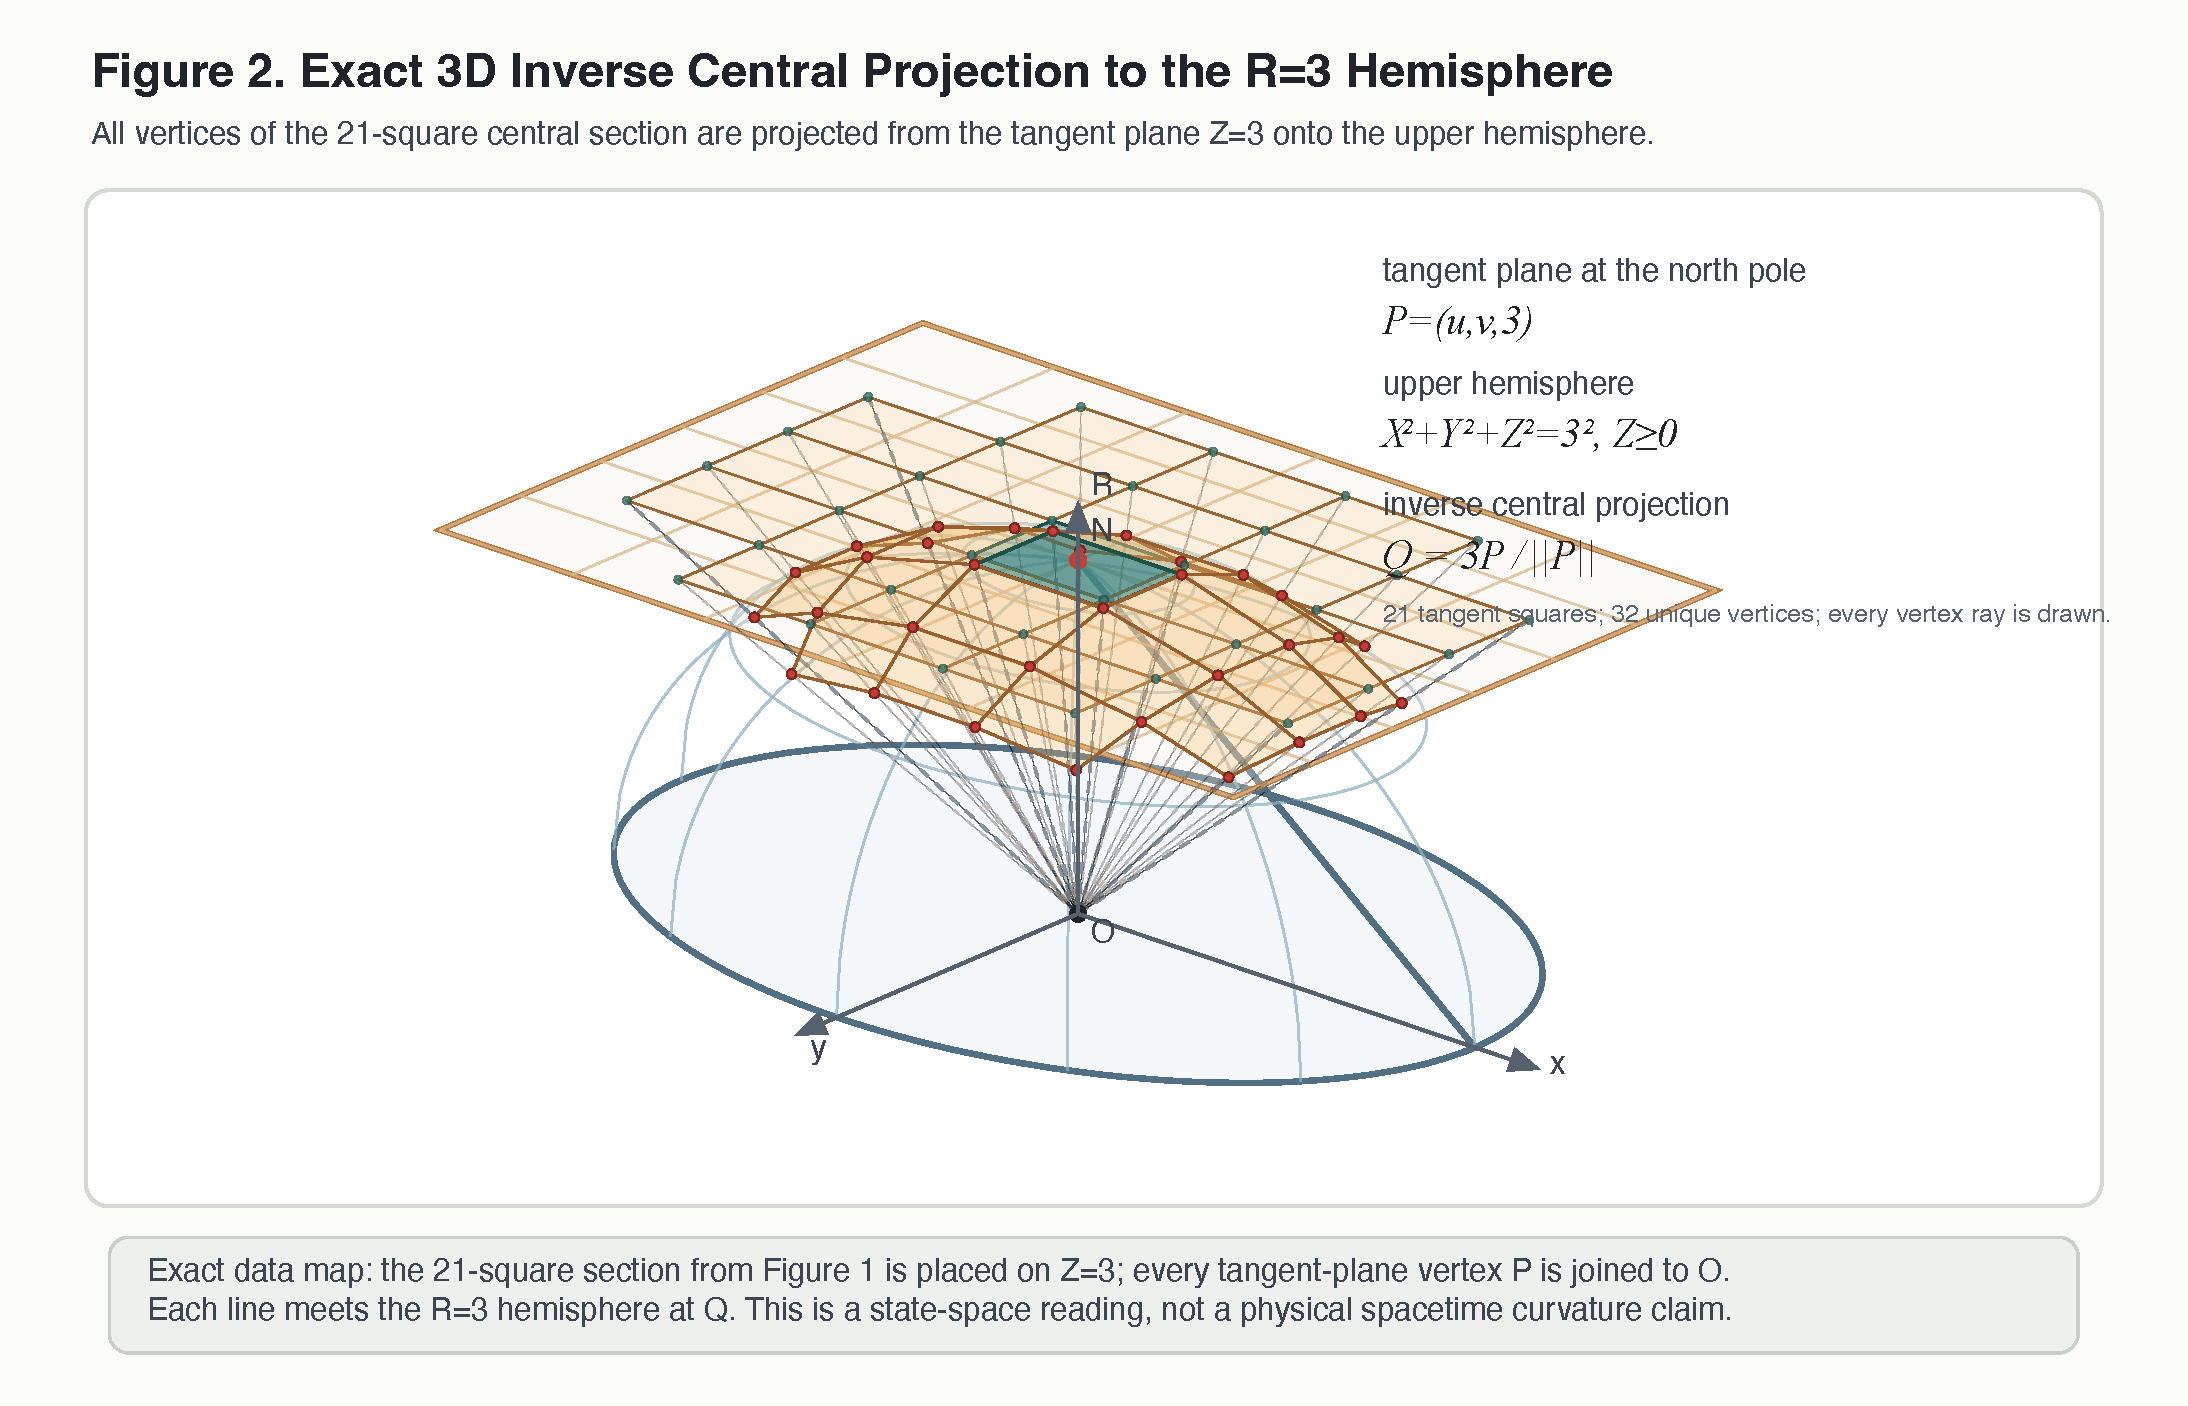
\includegraphics[keepaspectratio]{figure_paper4_2_radial_projection_curved_state_space.pdf}}
\caption{Figure 2. Exact 3D Inverse Central Projection to the R=3
Hemisphere}
\end{figure}

\textbf{Figure 2. Exact 3-dimensional inverse central projection from
the tangent plane to the hemisphere.} The 21 unit-square sections at the
right end of Figure 1 are read as a cell set on the \(xy\) plane tangent
to the north pole of the 3-dimensional hemisphere of radius \(R=3\). The
line connecting each vertex \(P=(u,v,3)\) on the tangent plane with the
center \(O\) intersects the hemisphere of radius 3 at exactly one point
\(Q=3P/\|P\|\). In the figure, this map is applied to all 32 vertices
obtained from the 21 squares. The reinterpretation into the curved state
space referred to in this paper is schematized as the inverse map of
central projection in this sense. However, this does not represent the
curvature of physical spacetime.

\subsubsection{9.3 Self-similar hierarchy}\label{self-similar-hierarchy}

When a state of some radius \(R\) is decomposed into a family of states
of finite radii \(R'_a\), each \(R'_a\) can in turn have internal
structure of the same form,

\[
{R'_a}^2=\sum_i \nu_{a,i}^2.
\]

Therefore, a hierarchy

\[
R\longrightarrow\{R'_a\}\longrightarrow\{R''_{a,b}\}\longrightarrow\cdots
\]

appears naturally.

We do not claim that this hierarchy is a figure with a strict fractal
dimension. However, in the sense that the same dual condition and the
same composite radius condition appear recursively at different scales,
it has a self-similar, or fractal-like, structure.

\begin{figure}
\centering
\pandocbounded{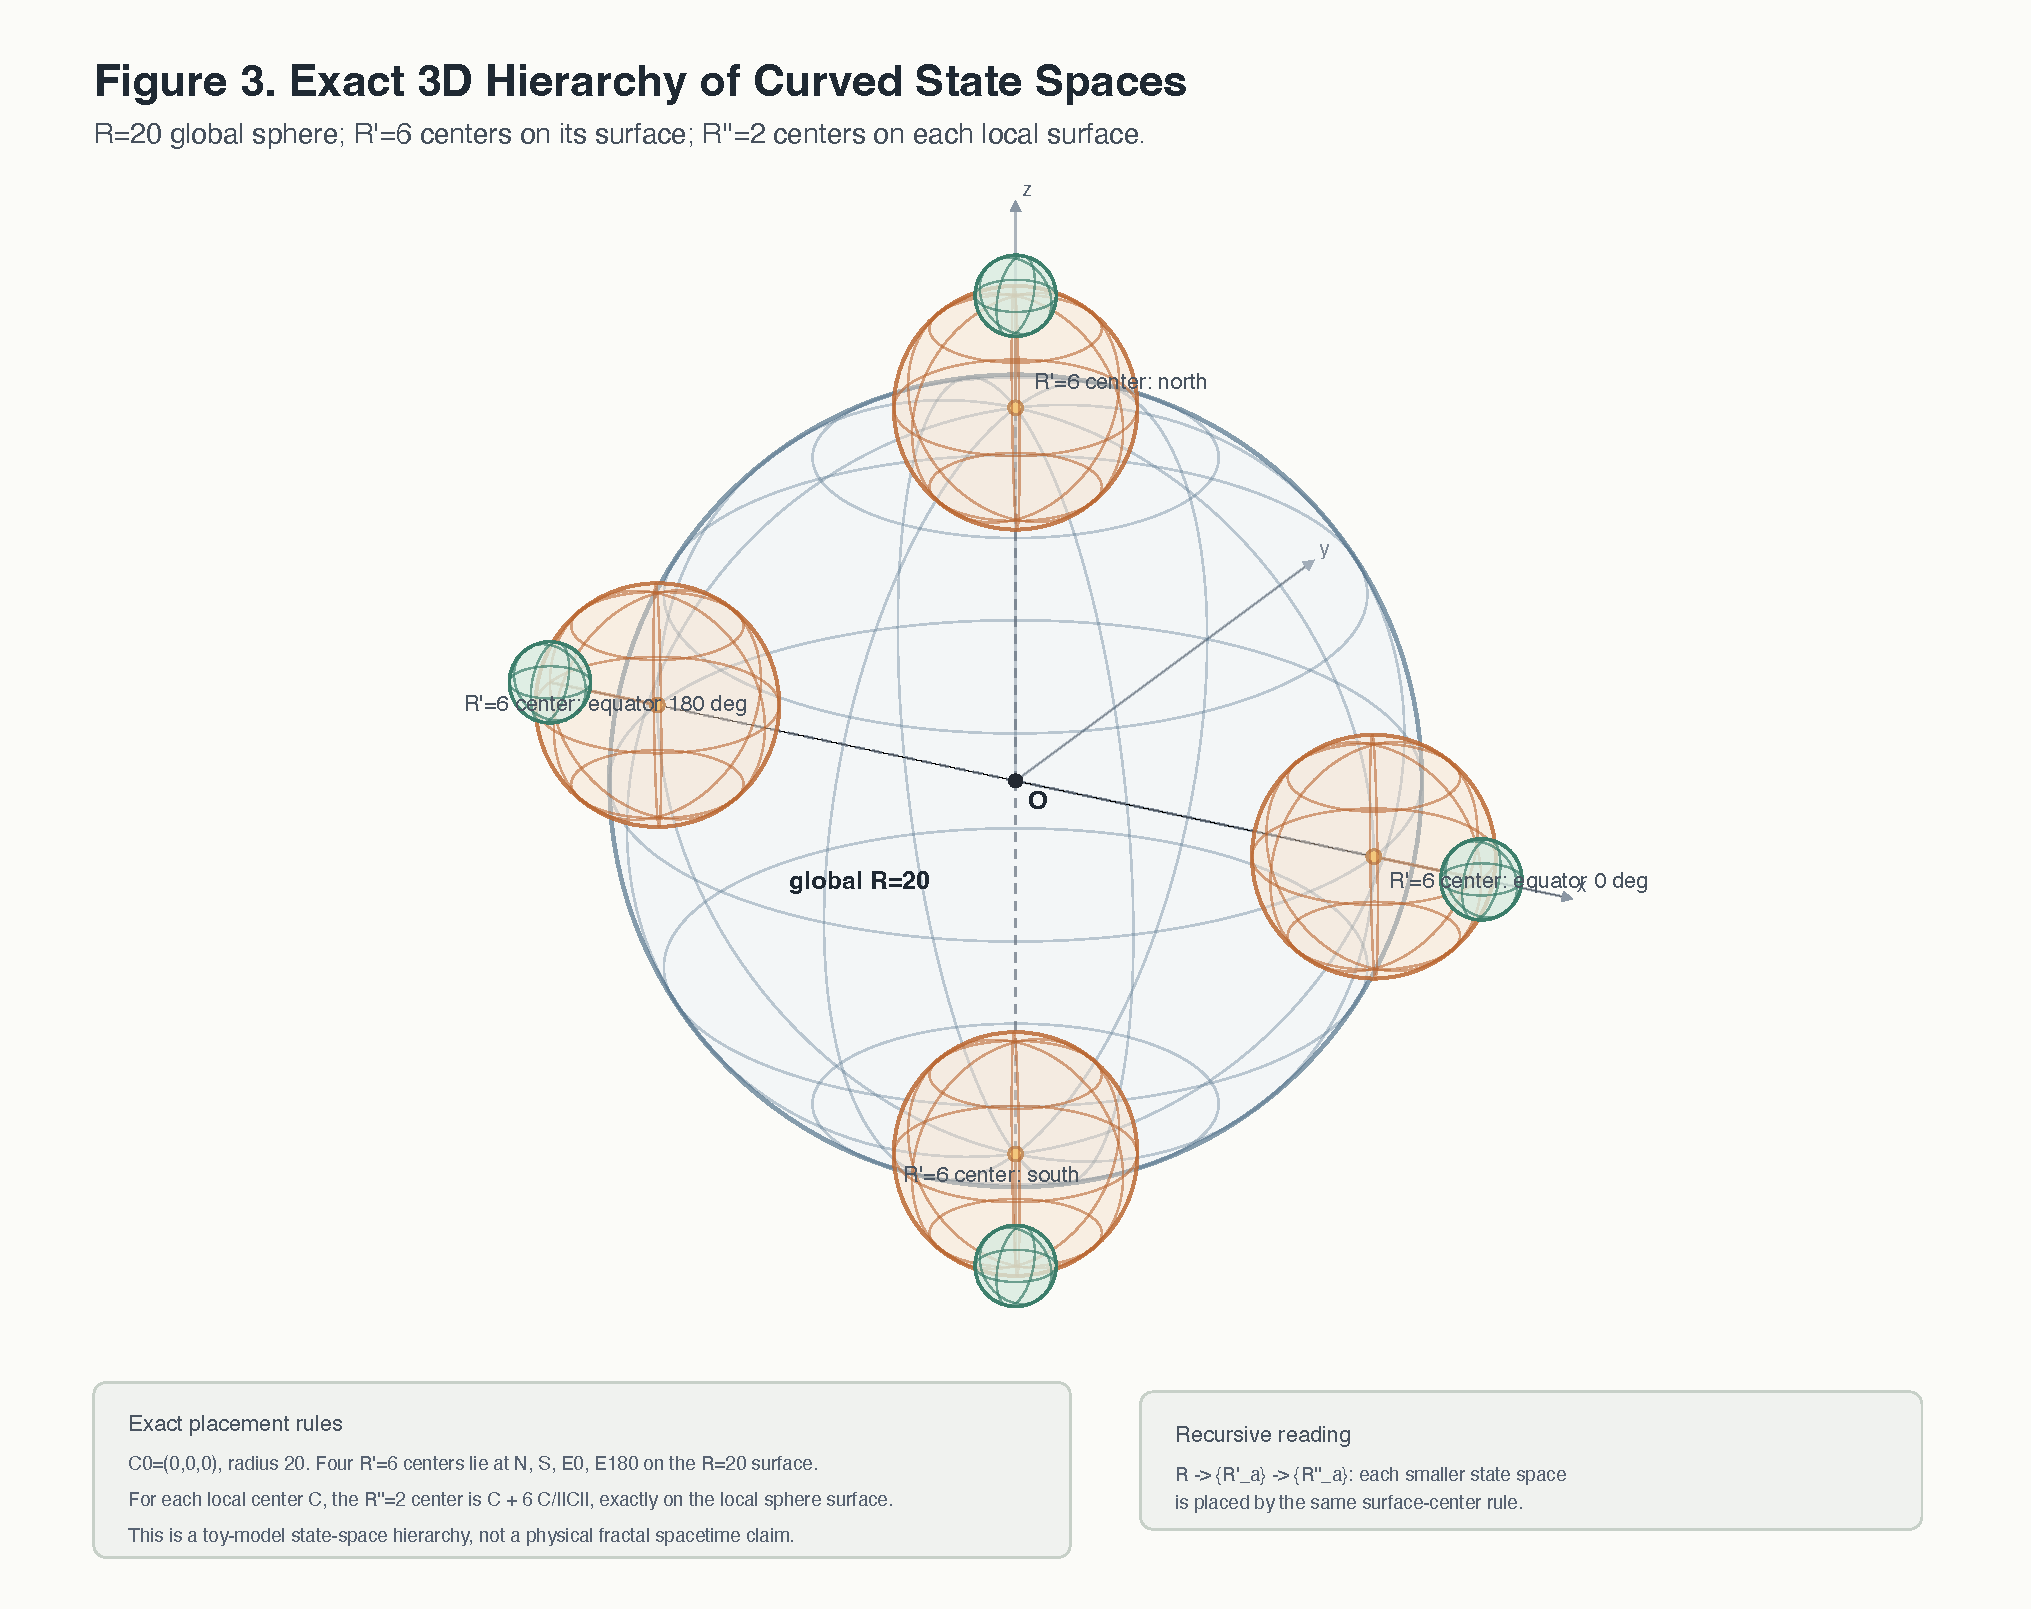
\includegraphics[keepaspectratio]{figure_paper4_3_hierarchical_curved_state_spaces.pdf}}
\caption{Figure 3. Hierarchical Curved State Spaces}
\end{figure}

\textbf{Figure 3. Exact 3-dimensional projection of hierarchical curved
state spaces.} A global sphere of radius \(R=20\) is placed, and local
spheres of radius \(R'=6\) are arranged centered at 4 points: its north
pole, south pole, and the points at \(0^\circ\) and \(180^\circ\) on the
equator. Furthermore, for each local sphere, a secondary sphere of
radius \(R''=2\) is placed centered at the surface point advanced from
the center \(C\) outward along the normal direction by \(6C/\|C\|\).
Thus the center of each \(R'=6\) sphere lies on the \(R=20\) sphere, and
the center of each \(R''=2\) sphere lies on the corresponding \(R'=6\)
sphere. This figure is a 3-dimensional projection of a toy model showing
the hierarchical placement rule, and does not claim that physical
spacetime is fractal.

\subsubsection{9.4 Observation as a curved
hierarchy}\label{observation-as-a-curved-hierarchy}

From the above, the state space of this model is not a simple lattice
cell set placed on a flat background. Rather, it is observed as a
hierarchical structure in which a curved state space contains smaller
curved state spaces, which in turn have internal structure of the same
form.

\begin{center}\rule{0.5\linewidth}{0.5pt}\end{center}

\subsection{10. Scope of Claims of This
Paper}\label{scope-of-claims-of-this-paper}

What this paper claims is limited to the following.

\begin{enumerate}
\def\labelenumi{\arabic{enumi}.}
\tightlist
\item
  From the reciprocal dual condition \(\lambda_n\nu_n=1\), a dual
  structure of wavelength space and frequency space can be defined.
\item
  Assuming a minimal conjugate width \(\delta_{\min}\), a state can be
  treated not as a point but as a minimal conjugate cell.
\item
  Via \(R^2=\sum_n\nu_n^2\), \(R\) can be read as a composite radius
  determined from the internal frequency components.
\item
  In the 4-dimensional fully-inscribed cell counting, \(N_0(1)=1\),
  \(N_0(2)=9\), \(N_0(3)=137\) appear.
\item
  \(R=1\) can be read as the minimal conjugate cell, \(R=2\) as 8
  first-neighbor quasi-ground states, and \(R=3\) as a large internal
  state shell containing 128 additional states.
\item
  The difference \(\Delta V(R)\) between the 4-dimensional hyperball
  volume \(V_4(R)\) and the cell volume \(N_0(R)\) corresponds to the
  boundary-layer volume and therefore grows mainly at order \(R^3\).
\item
  Reading the volume gap as a mismatch quantity, there are cases where a
  high-\(R\) state appears more consistent when decomposed into a family
  of finite-\(R'\) states.
\item
  After splitting, the \(\nu\) side appears to differentiate into
  internal state density and the \(\lambda\) side into extension and
  spread.
\item
  Connecting with central-projection-like observation, curved state
  spaces appear hierarchically and self-similarly.
\end{enumerate}

What this paper does not claim is as follows.

\begin{enumerate}
\def\labelenumi{\arabic{enumi}.}
\tightlist
\item
  This paper does not modify standard physics.
\item
  This paper does not derive general relativity, quantum theory, quantum
  field theory, or the Standard Model.
\item
  This paper does not prove the origin of time or space.
\item
  This paper does not derive physical constants, the elementary particle
  spectrum, interactions, gauge fields, or gravity.
\item
  This paper does not identify \(137\) with the fine-structure constant.
\item
  This paper does not derive the value of \(\delta_{\min}\).
\item
  This paper does not give a rigorous asymptotic expansion of the volume
  gap.
\item
  This paper does not assert cosmological reality.
\end{enumerate}

\begin{center}\rule{0.5\linewidth}{0.5pt}\end{center}

\subsection{11. Discussion}\label{discussion}

\subsubsection{11.1 Why complex structure appears from minimal
hypotheses}\label{why-complex-structure-appears-from-minimal-hypotheses}

The assumptions of this paper are very few. The central one is

\[
\lambda\nu=1,
\]

to which only the minimal conjugate width and the 4-dimensional cell
counting are added.

Nevertheless, the following structures appear in a chained manner:

\begin{itemize}
\tightlist
\item
  the minimal conjugate cell
\item
  internal state capacity
\item
  shell structure
\item
  the volume gap
\item
  consistency in splitting representations
\item
  the duality of global infinite radius and local finite radius
\item
  role differentiation between the \(\nu\) side and the \(\lambda\) side
\item
  curved hierarchical structure
\item
  self-similar decomposition
\end{itemize}

This shows that the reciprocal dual condition is not a mere algebraic
formula, but carries very strong constraints as a constitutive principle
of state space.

\subsubsection{11.2 Why it looks sparse}\label{why-it-looks-sparse}

Inside the state space, many finite-\(R'\) cells can exist. Viewed from
the frequency side, this appears as dense internal states.

However, on the wavelength side, by reciprocal duality they appear as
spread. Therefore, the same structure looks packed on the \(\nu\) side
and looks sparse on the \(\lambda\) side.

This observation provides a toy model that reads the vacuum not as
``empty space with nothing in it'' but as ``a state in which internal
states exist but appear on the wavelength side as a sparse extension.''

\subsubsection{11.3 Why this paper must be written
cautiously}\label{why-this-paper-must-be-written-cautiously}

The structure of this paper evokes associations with the differentiation
of time and space, vacuum structure, spacetime emergence, self-similar
cosmologies, and so on. However, asserting these directly would exceed
the verifiable scope of the model.

For this reason, this paper states only the observational structures
that appear from the minimal reciprocal dual condition. Room is left for
readers to examine possible physical correspondences, but this paper
itself makes no physical identification.

This caution is not a weakness of the model, but a condition for
enhancing its reusability.

\begin{center}\rule{0.5\linewidth}{0.5pt}\end{center}

\subsection{12. Conclusion}\label{conclusion}

In this paper, starting from the minimal reciprocal dual condition
placed between wavelength components \(\lambda_n\) and frequency
components \(\nu_n\),

\[
\lambda_n\nu_n=1,
\]

we organized the minimal conjugate width, the 4-dimensional
fully-inscribed cell counting, the volume gap, the finite-\(R'\)
decomposition, duality breaking, and the curved hierarchical structure
as a single observational model.

The main conclusions are as follows.

First, a state can be treated not as a point but as a minimal conjugate
cell centered at \(\nu=1,\lambda=1\). \(R=1\) can be read as the
ground-like state corresponding to this minimal conjugate cell.

Second, at \(R=2\) eight first-neighbor quasi-ground states appear, and
at \(R=3\) 128 additional states appear. This shows that the internal
state capacity grows rapidly with \(R\).

Third, by comparing the 4-dimensional hyperball volume with the
fully-inscribed cell volume, the filling fraction shows an
asymptotically increasing tendency accompanied by local fluctuations,
while the volume gap as an absolute quantity remains as a
boundary-layer-derived quantity of order \(R^3\). Reading this volume
gap as a mismatch quantity, there are cases where a high-\(R\) state
appears more consistent when decomposed into a family of finite, small
\(R'\) states.

Fourth, the post-splitting states are observed as dense internal states
on the \(\nu\) side and as a sparse extension on the \(\lambda\) side.
This can be read as a role differentiation of the wavelength-frequency
duality, that is, a structure analogous to spontaneous symmetry
breaking.

Fifth, \(R\) is not a radius given from outside but a composite quantity
determined from the internal frequency components. Therefore, an \(R\)
state can be decomposed into finite-\(R'\) states, and each \(R'\) state
can in turn have internal structure of the same form. In this sense,
this model has a curved, self-similar hierarchical structure.

This paper does not claim a unified physical theory. However, it is a
reusable toy observation model showing that, from the minimal assumption
\(\nu\lambda=1\), the internal state capacity, the volume gap, splitting
representations, duality breaking, and curved hierarchical structure can
be read in a chained manner.

\begin{center}\rule{0.5\linewidth}{0.5pt}\end{center}

\subsection{Appendix A: Definition of the Fully-Inscribed Cell
Counting}\label{appendix-a-definition-of-the-fully-inscribed-cell-counting}

Consider the unit cell of side 1 associated with the 4-dimensional
lattice point

\[
k=(k_1,k_2,k_3,k_4)\in\mathbb{Z}^4.
\]

The half-width in each direction is \(1/2\). For the whole unit cell to
be fully inscribed in the 4-dimensional hyperball of radius \(R\), it
suffices that the farthest vertex of the cell lies within radius \(R\).

Therefore the condition is

\[
\sum_{i=1}^{4}\left(|k_i|+\frac12\right)^2\le R^2.
\]

The fully-inscribed cell count is defined by

\[
N_0(R)=\#\left\{k\in\mathbb{Z}^4\mid
\sum_{i=1}^{4}\left(|k_i|+\frac12\right)^2\le R^2
\right\}.
\]

\begin{center}\rule{0.5\linewidth}{0.5pt}\end{center}

\subsection{Appendix B: Python Code for
Reproduction}\label{appendix-b-python-code-for-reproduction}

The following is minimal code that computes \(N_0(R)\), the
4-dimensional hyperball volume, the volume gap, and the filling fraction
for integer radii \(R=1\) to \(R=10\).

\begin{Shaded}
\begin{Highlighting}[]
\ImportTok{import}\NormalTok{ math}
\ImportTok{import}\NormalTok{ itertools}

\KeywordTok{def}\NormalTok{ N0(R):}
\NormalTok{    M }\OperatorTok{=} \BuiltInTok{int}\NormalTok{(math.ceil(R))}
\NormalTok{    count }\OperatorTok{=} \DecValTok{0}
    \ControlFlowTok{for}\NormalTok{ k }\KeywordTok{in}\NormalTok{ itertools.product(}\BuiltInTok{range}\NormalTok{(}\OperatorTok{{-}}\NormalTok{M, M }\OperatorTok{+} \DecValTok{1}\NormalTok{), repeat}\OperatorTok{=}\DecValTok{4}\NormalTok{):}
\NormalTok{        s }\OperatorTok{=} \BuiltInTok{sum}\NormalTok{((}\BuiltInTok{abs}\NormalTok{(x) }\OperatorTok{+} \FloatTok{0.5}\NormalTok{)}\OperatorTok{**}\DecValTok{2} \ControlFlowTok{for}\NormalTok{ x }\KeywordTok{in}\NormalTok{ k)}
        \ControlFlowTok{if}\NormalTok{ s }\OperatorTok{\textless{}=}\NormalTok{ R}\OperatorTok{*}\NormalTok{R }\OperatorTok{+} \FloatTok{1e{-}12}\NormalTok{:}
\NormalTok{            count }\OperatorTok{+=} \DecValTok{1}
    \ControlFlowTok{return}\NormalTok{ count}

\NormalTok{prev }\OperatorTok{=} \DecValTok{0}
\ControlFlowTok{for}\NormalTok{ R }\KeywordTok{in} \BuiltInTok{range}\NormalTok{(}\DecValTok{1}\NormalTok{, }\DecValTok{11}\NormalTok{):}
\NormalTok{    n }\OperatorTok{=}\NormalTok{ N0(R)}
\NormalTok{    shell }\OperatorTok{=}\NormalTok{ n }\OperatorTok{{-}}\NormalTok{ prev}
\NormalTok{    V4 }\OperatorTok{=}\NormalTok{ (math.pi}\OperatorTok{**}\DecValTok{2} \OperatorTok{/} \FloatTok{2.0}\NormalTok{) }\OperatorTok{*}\NormalTok{ R}\OperatorTok{**}\DecValTok{4}
\NormalTok{    gap }\OperatorTok{=}\NormalTok{ V4 }\OperatorTok{{-}}\NormalTok{ n}
\NormalTok{    eta }\OperatorTok{=}\NormalTok{ n }\OperatorTok{/}\NormalTok{ V4}
    \BuiltInTok{print}\NormalTok{(R, n, shell, V4, gap, eta)}
\NormalTok{    prev }\OperatorTok{=}\NormalTok{ n}
\end{Highlighting}
\end{Shaded}

\begin{center}\rule{0.5\linewidth}{0.5pt}\end{center}

\subsection{References}\label{references}

{[}1{]} Noriaki Kihara, ``Paper 1: Dual Geometry of Wavelength Space and
Frequency Space --- A Geometric and Topological Observational Model of
Reciprocal Conditions, Logarithmic Representation, and
Uncertainty-Weighted Counting,'' v0.3, 2026. DOI:
10.5281/zenodo.20588037. Concept DOI: 10.5281/zenodo.20588036.

{[}2{]} Noriaki Kihara, ``Paper 2: Radius Sweep of Fully-Inscribed
Unit-Cell Counts on a 4-Dimensional Lattice --- An Enumeration Table
from R = 0.5 to 10.0 with a Reproducible Formulation,'' v0.2, 2026. DOI:
10.5281/zenodo.20607574. Concept DOI: 10.5281/zenodo.20588038.

{[}3{]} Noriaki Kihara, ``Paper 3: Closed Four-Degree-of-Freedom
Structure and Its Correspondence with 4-Dimensional Lattice Counting ---
A Geometric Organization from the 5-Component Sum-of-Squares Constraint
to the Unit-Cell Counting Region,'' v0.3, 2026. DOI:
10.5281/zenodo.20589515. Concept DOI: 10.5281/zenodo.20589261.

{[}4{]} Sumati Surya, ``The causal set approach to quantum gravity,''
Living Reviews in Relativity 22, 5 (2019). arXiv:1903.11544.

{[}5{]} Tomasz Konopka, Fotini Markopoulou, Simone Severini, ``Quantum
Graphity: a model of emergent locality,'' Physical Review D 77, 104029
(2008). arXiv:0801.0861.

{[}6{]} Tomasz Konopka, Fotini Markopoulou, ``Quantum Graphity,''
arXiv:hep-th/0611197 (2006).

{[}7{]} Daniele Oriti, ``Tensorial Group Field Theory condensate
cosmology as an example of spacetime emergence in quantum gravity,''
arXiv:2112.02585 (2021).

{[}8{]} A. G. A. Pithis, M. Sakellariadou, ``Group field theory
condensate cosmology: An appetizer,'' Universe 5(6), 147 (2019).
arXiv:1904.00598.

{[}9{]} Christof Wetterich, ``Pregeometry and spontaneous time-space
asymmetry,'' arXiv:2101.11519 (2021).

{[}10{]} G. E. Volovik, \emph{The Universe in a Helium Droplet}, Oxford
University Press, 2003.

\begin{center}\rule{0.5\linewidth}{0.5pt}\end{center}

\subsection{License}\label{license}

This paper is published under CC BY 4.0.\\
Reuse, adaptation, translation, and citation are permitted, provided
that the author name, version, publication date, and source are clearly
indicated.

\end{document}
